\documentclass[a4paper,12pt,titlepage]{article}
\usepackage[polish,english]{babel}
\usepackage[utf8]{inputenc}
\usepackage[T1]{fontenc}
\usepackage{tabularx}
\usepackage[pdftex]{graphicx}
\usepackage{amsmath}
\usepackage{geometry}
\geometry{lmargin=3cm,rmargin=3cm,tmargin=3cm,bmargin=3cm}
\title{Physics of The Critical Point\\\normalsize Cluster Frequency in 1D and 2D Ising Model\\\small Summation of co-op part of project}

\author{Kamil Kaczmarczyk \\ Mariusz Jędraczka}
\begin{document}
\maketitle
\newpage
  \section{Introduction}
  When considering Ising model one is mostly interested in properties like energy, susceptibility, magnetization, etc. All this 
  parameters are very interesting and useful but observation of the given model, its evolution and characteristic behavior is as much
  interesting itself and of course connected with other properties.
  
  Simple anticipations about 1D or 2D Ising model of spins are quite obvious. We are interested in evolution of our spin system through
  temperature. Since energy of each spin is directly connected with the temperature of the system we can assume that with its lowering
  energy of whole lattice will decrease. Spins will tend to form groups of spins oriented in paralell direction - clusters. The growing
  order of spin lattice is quite interesting because it undergoes similar distribution in each dimension.
  
  We agree that with $T \rightarrow \infty$ clusters size (number of paralell spins in neighbourhood) grows. The parameter describing
  this behavior is called correlation length $\xi$.
  
  
  We can connect it with other parameters of the system in following ways. First approach considers correlation between spins and relation between correlation lenght is as given
  below.
  \begin{equation}
   \left<\sigma_i,\sigma_j\right>\sim e^{-\frac{|i-j|}{\xi}}
  \end{equation}
  In fixed temperature correlation length is the inverse factor in exponent index of spin correlation function versus correlation distance.
  In our simmulation we used this relation to determine $\xi$ parameter, for given temperature.
  
  To measure mean cluster size in fixed temperature we used simple function to count spins that belong to each cluster and take its mean
  value over number of Monte Carlo cycles. Below we present equations claryfing this topic.
  
  Firstly consider one chain of $N$ spins in fixed temperature (or lattice in 2D, it is irrelevant). Let's assume some distribution
  of clusters. If cluster of size $s$ has appeared $k$-times we can write down probability of observing this cluster:
  \begin{displaymath}
   P_s=\frac{s \cdot k}{N}
  \end{displaymath}
  One can simply check that if we make sum over all observed cluster we will get $P=1$ - probability of observing any cluster, it is
  obviously equal $1$. Now we can move to writing down equation for mean cluster size $\left<S\right>$. From definition of mean value of observable we get:
  \begin{displaymath}
   \left< S\right> = \sum_{s=1}^{N}sP_s=\frac{\sum_{s=1}^{N}{s^2k_s}}{N}
  \end{displaymath}
  where $k_s$ is the number of clusters of size $s$ observed for given spin chain.
  
  If we allow to evolve our system $t$ times and increase accordingly $k_s$ we will get mean value of cluster size by dividing additionaly
  by $t$.
  
  This two parameters - correlation length and mean cluster size - were used to make plot to check the relation between them which we
  expect to be linear.
  \begin{displaymath}
   \left< S \right> \sim \xi
  \end{displaymath}

  \section{Simulations results}
  Firstly we want to present behavior of size cluster versus temperature for 1D and 2D Ising model. To make Monte Carlo simulations
  we used Wolf algorythm for both dimensions. To take mean value we made $100$ MC cycles in each temperature.
  
  \begin{figure}[h]
    \centering
    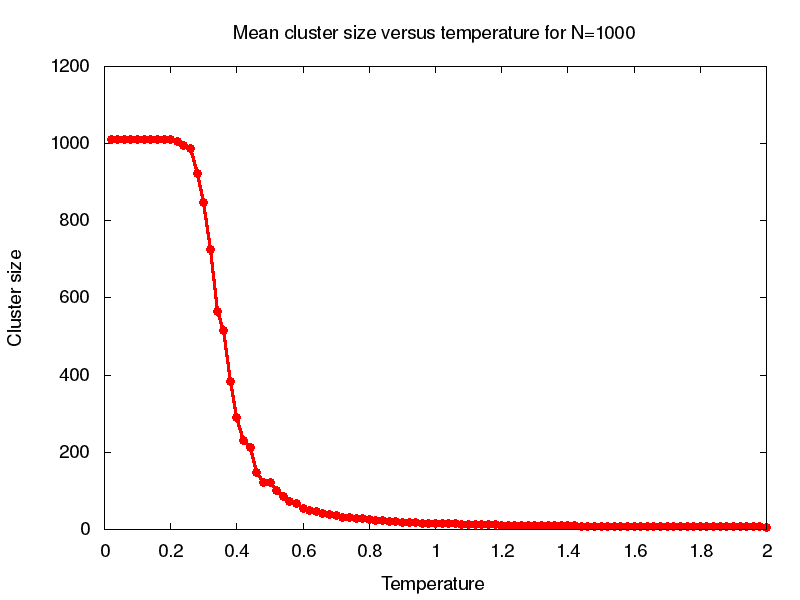
\includegraphics[scale=0.5]{plots/IsingTestMeanClusterFreq1D.png}
  \end{figure}
  
  This plot corresponds to 1D model of $1000$ spins. As one can see spins are quite long (in temperature scale) in chaotic state. At relatively short
  distance they start to merge with eachother just to form one big paralell oriented spins.
  
  \newpage
  \begin{figure}[h]
    \centering
    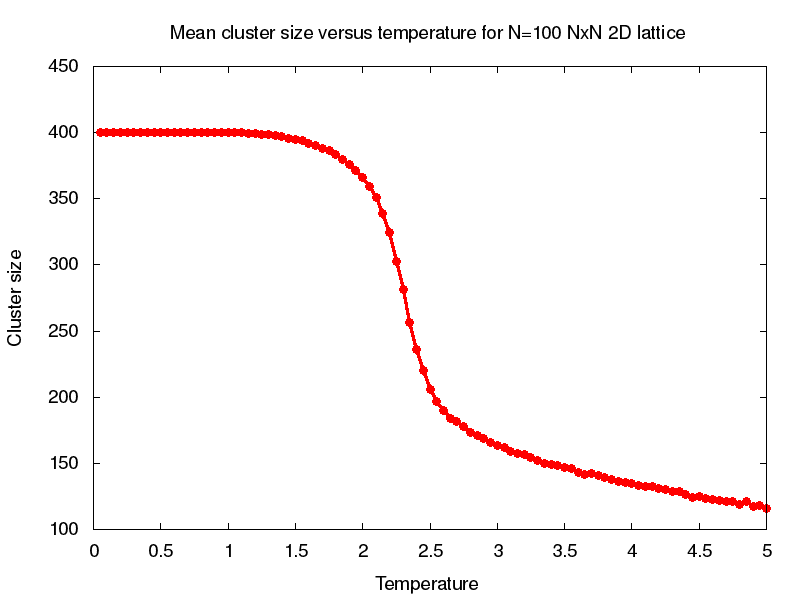
\includegraphics[scale=0.5]{plots/IsingTestMeanClusterFreq2D.png}
  \end{figure}
  
  2D model simulations were performed on $20\times20$ lattice. It needs to be denoted that in low temperature close to $0$ our model 
  is ineficient for both dimensions. It corresponds to the case where whole lattice is one, big cluster. Specialy Metropolis algorythm shows its weakness in
  low temperatures, it is connected to correlation time but for that topic we send to appropriate section of this project.
  \newpage
  Additionaly we prepeared few pictures of spin lattice in different temperautre to show
  how cluters are growing with lowering the temperature. Since this simulations were much faster due to its simplicity we used $100\times 100$ lattice
  and Wolf algorythm, this is like snapshot of the lattice so there are no mean values and additional parameters of clusters since one
  can see with his own eyes whole process.
  
  \begin{figure}[th]
    \centering
    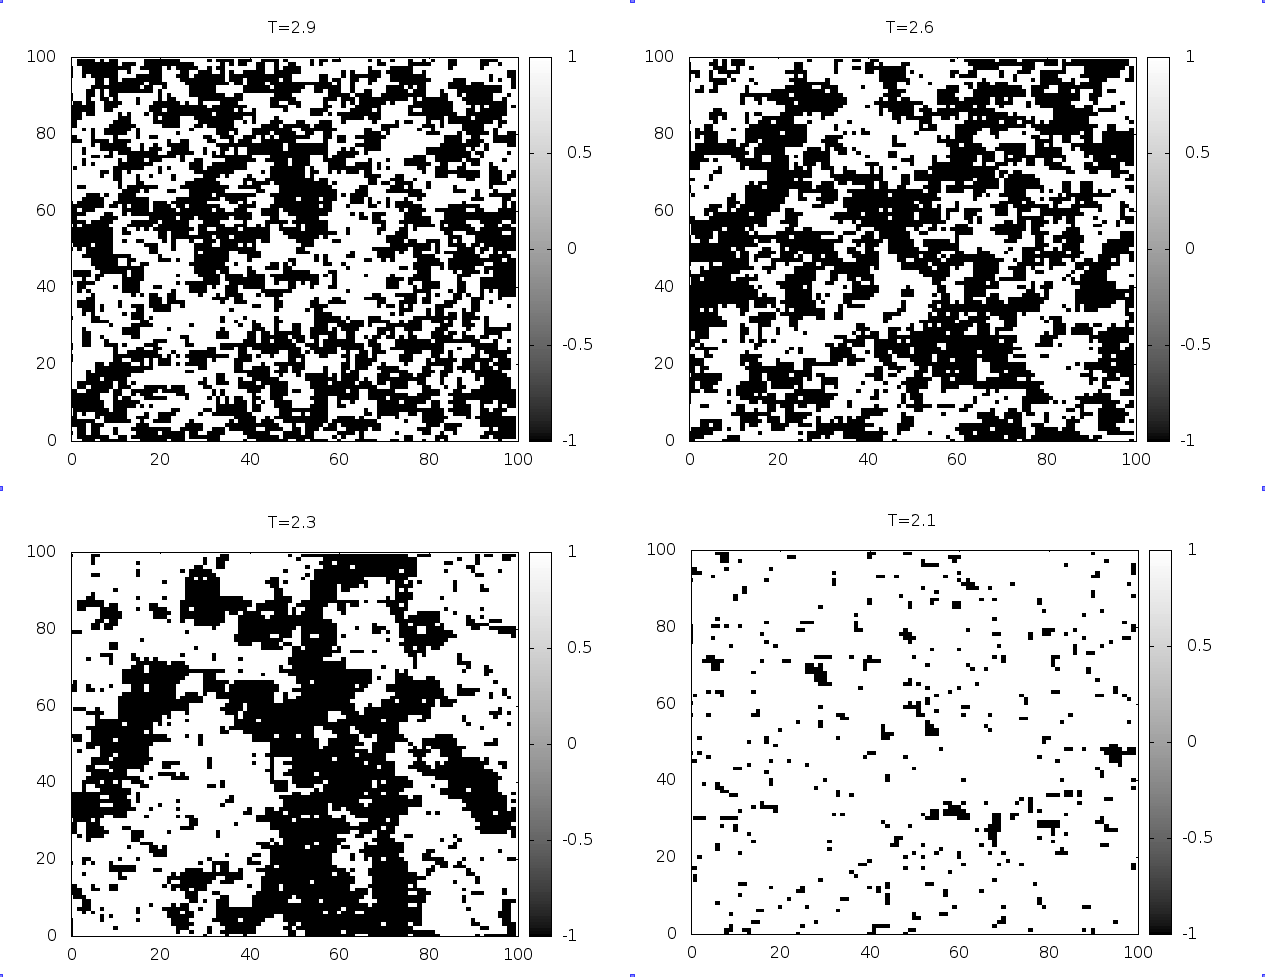
\includegraphics[scale=0.36]{plots/2DLattice.png}
  \end{figure}
 \newpage
  To check relation between mean cluster size an correlation length we will used 1D model. As one can see first variable is easy
  to obtain but to determine $\xi$ for given temperature we have to fit exponential function of spin-spin correlation function. We place
  as example plot of this function for one temperature. We wanted to take 10 values of $\xi$ and it would be problematic to place all
  10 plots in this document so only data will be presented.
  \begin{figure}[th]
    \centering
    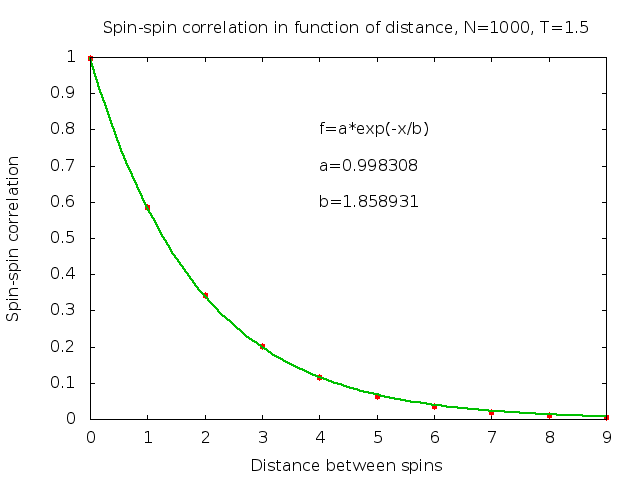
\includegraphics[scale=0.5]{plots/IsingTestCorrelationLength.png}
  \end{figure}
  
  As one can see it is easy to obtain correlation length which is, according to the plot above, parameter $b$ in fit function, so for
  temperature $1.5$ : $\xi\approx 1.85893$.
  
  Now we present relation between mean cluster frequency and correlation length $\xi$ for temperatures in range of $\left[1.5,0.6\right]$.
  \begin{figure}[th]
    \centering
    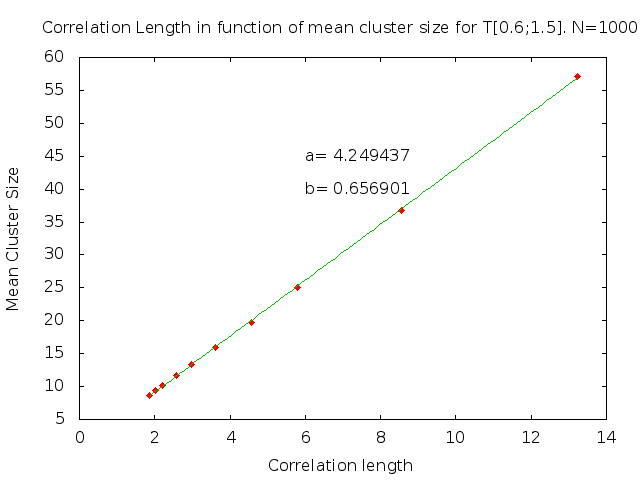
\includegraphics[scale=0.49]{plots/IsingTestCLvsMCS.png}
  \end{figure}
  
  Fit of measured point shows very clear linear relation. As one can see temperatures are ranging from $0.6$ to $1.5$, which we consider
  safe in the matter of functionality of our model. All of above simulations were made using Wolf algorythm and with respect to correlation
  time - for this algorythm it was of $10^2$ order in low temperatures so our calculations included rather low frequency measurements.
  
\end{document}